\documentclass{beamer}
\usepackage{media9}
%\usepackage{movie15}


%\usepackage{graphicx}
\usepackage{verbatim}

\useoutertheme{shadow}
%\usecolortheme{orchid}
\usecolortheme{seahorse}

\renewcommand{\a}{\alpha}
\renewcommand{\b}{\beta}
\renewcommand{\d}{\delta}
\newcommand{\g}{\gamma}
\newcommand{\s}{\sigma}
\newcommand{\w}{\omega}
\renewcommand{\k}{\vec{k}}
\newcommand{\td}[1]{\tilde{#1}}
\newcommand{\x}{\vec{x}}
\newcommand{\p}{\phantom{\alpha}}

\def\toonscale{0.45}
\def\mboxy#1{\mbox{\small #1}}


\begin{comment}
\AtBeginSection[]{
  \frame{
    \frametitle{Outline}
    \tableofcontents[currentsection]
  }
}
\end{comment}

\title{PTA Confusion}
\subtitle{Resolution, Source Confusion and Stochasticity in Pulsar Timing Arrays}
\author[Boyle and Pen]{Ue-Li Pen, Latham Boyle ++ \\[8mm] 
}
\date{IPTA 2018, June 22, 2018}


\begin{document}

\frame{\titlepage}

%\section*{Introduction}
\section{Introduction}

\begin{comment}
  \subsection{Outline}

  \frame{
    \frametitle{Outline}
    \tableofcontents
  }
\end{comment}

  \subsection{PTA}
  \frame{
    \frametitle{Redshift maps}
    \begin{itemize}
      \item overcoming 'confusion limit'
      \item redshift maps: Boyle+UP 2012, Roebber+Holder 2017
      \item Densely sampled limit
      \item ToA map: angle+time data cube
      \item FFT into complex 2-D map at each frequency
    \end{itemize}
  }
\section{Gravity Wave Image}

  \frame{
    \frametitle{Redshift Image}
%    \begin{minipage}{0.6\linewidth}
    \vspace{-0.2in}
    \begin{itemize}
    \item \mboxy{$\delta t = \sin(2\phi)[1+\cos(\theta)]$}
    \end{itemize}
%    \end{minipage}
    \begin{minipage}{0.35\linewidth}
%      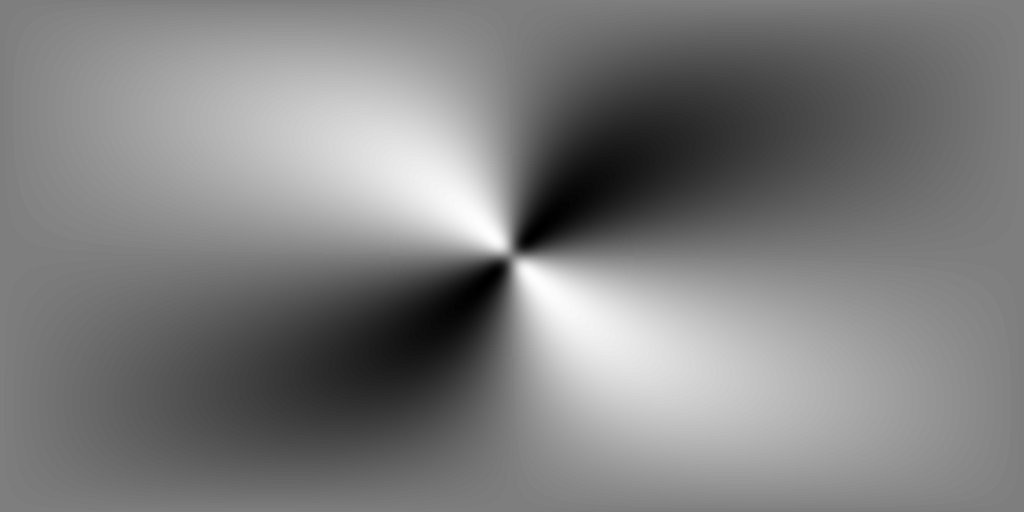
\includegraphics[scale=0.25]{Figures/residual}
%\visible{\includemovie[poster,text={\small(Loading
%    Video...)}]{6cm}{4cm}{Figures/residual.mp4}}

\includemedia[
  label=some_dice,
  width=3.0\linewidth,height=1.35\linewidth, % 16:9
  addresource=Figures/residual.mp4, 
  addresource=Figures/residual1.mp4, 
  transparent,
  activate=pageopen,
  passcontext,
  flashvars={
    source=Figures/residual.mp4
   &autoPlay=true % start playing on activation
   &loop=true
  }
]{}{VPlayer.swf} 
% loop video
\mediabutton[
  mediacommand=some_dice:playPause,
  overface=\color{blue}{\fbox{\strut Play/Pause}},
  downface=\color{red}{\fbox{\strut Play/Pause}}
]{\fbox{\strut Play/Pause}}
\mediabutton[
  mediacommand=some_dice:setSource [(Figures/residual1.mp4)]
]{\fbox{\strut Face-on
}}


    \end{minipage}
    \hspace{0.02\linewidth}
    
        singular spatial structure near GW source, no residual in
    anti-direction (TT).  

    }


  \frame{
    \frametitle{Two sources}
      \vspace{0.5cm}
      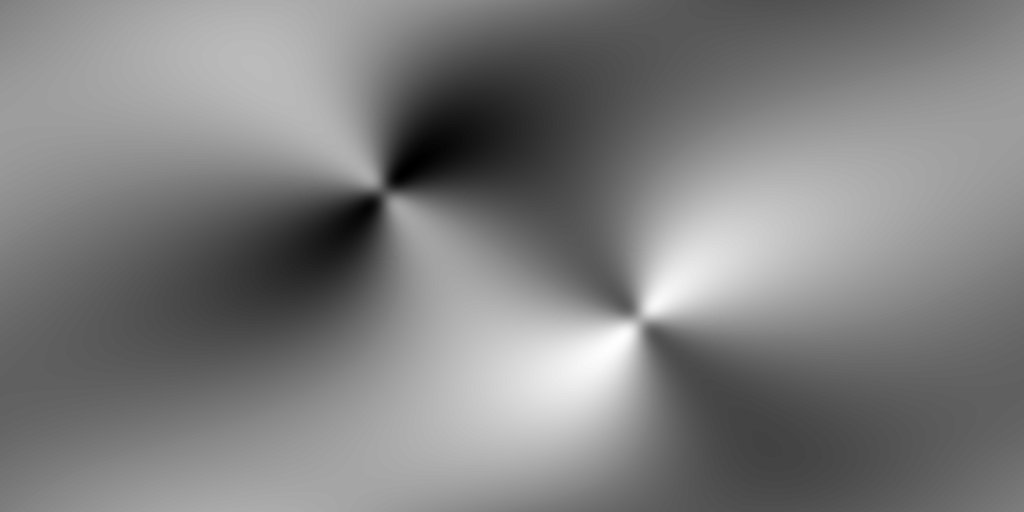
\includegraphics[scale=0.32]{Figures/residual2}
    \begin{itemize}
      \item Well resolved by dense PTA
    \end{itemize}
    }



  \subsection{2-D}

  \frame{
    \frametitle{Background}
    \begin{itemize}
      \item traditional technique: measure 2 point correlation
        function of residuals (Hellings-Downs, Jenet, etc).
      \item equivalent to power spectrum
      \item results in unintended source confusion, 'stochastic
         background'
       \item sell as 'pulsar GW imaging array'
    \end{itemize}
  }


\subsection{Residual}
\frame{
  \frametitle{Formulation}
TT gauge line element:
\begin{equation}
  \label{metric}
  ds^{2}=-dt^{2}+[\delta_{ij}+2h_{ij}]dx^{i}dx^{j}.
\end{equation}
In this gauge, the $\vec{x}={\rm constant}$ worldlines are timelike
geodesics; along such a worldline, the proper time $\tau$ is just the
coordinate time $t$.   Single gravitational
plane wave travelling in the $\hat{n}$ direction
\begin{equation}
  \label{deltat(omega)}
  \delta \tilde{t}_{\alpha}(\omega)=\frac{i}{\omega}
  \frac{\tilde{h}_{ij}(\omega)\hat{r}_{\alpha}^{i}\hat{r}_{\alpha}^{j}
    [1-{\cal P}_{\alpha}(\omega)]}{(1\!+\!\hat{n}\!\cdot\!\hat{r}_{\alpha})}
\end{equation}
with phase
\begin{equation}
  \label{P_alpha}
  {\cal P}_{\alpha}(\omega)\equiv
  {\rm e}^{i\omega r_{\alpha}(1+\hat{n}\cdot\hat{r}_{\alpha})}.
\end{equation}
reduces to $\delta t = \sin(2\phi)[1+\cos(\theta)]$ when averaging
over all pulsar distances.  Well known result.
}



  \subsection{Finite Corrections}

  \frame{
    \frametitle{Distance}
    \begin{itemize}
    \item At angles $\theta < \sqrt{\frac{\lambda_{\rm GW}}{r}}$ the
      intrinsic pulsar delay cancels the earth delay
    \item Typical distances $r \sim$ kpc, $\lambda_{\rm GW} \sim 3 $ pc,
      $\theta \sim 5^o$
    \item Confused if more than 100's of sources, or more sources than
      pulsars. 
    \end{itemize}
  }
      

%  \subsection{Statistics}

  \section{3-D imaging}
  \subsection{GW interferometry}
  \frame{
    \frametitle{3-D}
    \begin{itemize}
      \item if distances to pulsars are known to better than 1
        wavelength ($\sim$pc), source positions are known to $\delta \theta \sim
        \frac{\lambda}{D}$.
      \item arc minute localization: much more precise than LIGO++
      \item complications when pulsar period changes over the 3-D
        extent of PTA
    \end{itemize}
  }

  \frame{
    \frametitle{Distance measurement}
    \begin{itemize}
    \item VLBI Scintillometry: demonstrated 50 pico arcsecond astrometry
      (Pen++2014)
    \item ongoing test in known systems
    \item promising for binary systems
    \item low frequency VLBI monitoring: LWA, LOFAR, GMRT, MWA, etc
    \end{itemize}
  }

  \subsection{Conclusions}
  \frame{
    \frametitle{Conclusions}
    \begin{itemize}
    \item PTA has potential to be high resolution GW telescope    
    \item 3-D: $\sim \frac{10'}{\rm SNR}$
    \item Changes physical interpretation of PTA GW signals: unlikely
      to be in stochastic regime.  2-PCF confusion analysis is
      self-fulfilling prophecy.
    \item sellable feature: orders of magnitude more precise in angle than LIGO
    \item motivation for precision pulsar VLBI scintillometry
      distances
    \item Scintillometry 2018: Oct 22-26 at TDLI in Shanghai!
    \end{itemize}
  }
\end{document}
